% ==========================================
% PLANTILLA LATEX — DOCUMENTOS ACADÉMICOS
% ==========================================
%
% CÓMO USAR ESTA PLANTILLA:
%   1. Edita  config/proyecto.tex   con los datos de tu proyecto
%   2. Crea tus capítulos en  capitulos/
%   3. Descomenta los \input que necesites abajo
%   4. Compila:  latexmk -pdf -outdir=build main.tex
%
% ESTRUCTURA DE CARPETAS:
%   config/       → Configuración (editar sólo proyecto.tex)
%   common/       → Archivos estáticos de la plantilla (no tocar a menos que sepas lo que haces)
%   capitulos/    → Tus capítulos (tu contenido va aquí)
%   imagenes/     → Imágenes (logos en imagenes/logos/)
%   build/        → Salida de compilación (se genera solo)
%
% TIP: Si algo no compila, limpia build/ y reintenta:
%      latexmk -C -outdir=build ; latexmk -pdf -outdir=build main.tex
%
% ==========================================

\documentclass[11pt, letterpaper]{report}

% --- Datos del proyecto (EDITAR ESTE ARCHIVO) ---
% ==========================================
% CONFIGURACIÓN DEL PROYECTO
% ==========================================
%
% Este es el ÚNICO archivo que necesitas editar para
% personalizar la plantilla a tu proyecto.
%
% TIP: No modifiques archivos en common/ ni config/configuracion.tex
%      a menos que necesites funcionalidad avanzada.
%
% TIP: Los campos marcados con (*) son obligatorios.
%      Los demás puedes dejarlos vacíos con {}
% ==========================================

% --- Información del documento (*) ---
\newcommand{\titulo}{Práctica 2}
\newcommand{\subtitulo}{ Análisis y diseño de programas paralelos utilizando procesos}
\newcommand{\materia}{Cómputo paralelo}
\newcommand{\profesor}{}                   % Ej: Dr. Juan Pérez
\newcommand{\fechaEntrega}{24 de febrero del 2026}  % Cambiar por la fecha real

% --- Información institucional (*) ---
\newcommand{\institucion}{Instituto Politécnico Nacional}
\newcommand{\escuela}{Escuela Superior de Cómputo}
\newcommand{\siglasEscuela}{ESCOM}         % Siglas de la escuela
\newcommand{\carrera}{Ingeniería en Inteligencia Artificial}
\newcommand{\grupo}{6BV1}
\newcommand{\lugar}{Ciudad de México}       % Lugar de entrega

% --- Autores (*) ---
% TIP: Agrega o elimina líneas según el número de integrantes.
%      Si es trabajo individual, deja un solo nombre.
%      Separa cada nombre con \\
\newcommand{\listaAutores}{
    Bustillos Cruz Jonatan \\
    Delgado Lucero Cristian Isaac \\
    Frem Cortés José Angel \\
    Luna Gonzales Gabriel Alexis
}

% --- Logos ---
% TIP: Coloca tus logos en imagenes/logos/
%      Si no necesitas algún logo, déjalo vacío {}
\newcommand{\logoIzquierdo}{imagenes/logos/ipn_logo.png}
\newcommand{\logoDerecho}{imagenes/logos/escom_logo.png}

% --- Configuración de fuentes (opcional) ---
% TIP: Configura la fuente y tamaños de texto para el documento
%      Por defecto usa Times New Roman
%      Puedes cambiar los tamaños según tus necesidades

% Usar Times New Roman (true) o fuente por defecto (false)
\newcommand{\usarTimesNewRoman}{true}      % true o false

% Tamaños de fuente
\newcommand{\tamanoTextoBase}{11pt}        % Tamaño del texto normal
\newcommand{\tamanoTituloUno}{16pt}        % Tamaño para \chapter o nivel 1
\newcommand{\tamanoTituloDos}{14pt}        % Tamaño para \section o nivel 2
\newcommand{\tamanoTituloTres}{12pt}       % Tamaño para \subsection o nivel 3


% --- Paquetes y estilos (no tocar a menos que sepas lo que haces) ---
% ==========================================
% CONFIGURACIÓN DE LA PLANTILLA
% ==========================================
%
% ADVERTENCIA: Este archivo contiene la configuración base
% de paquetes y estilos. Normalmente NO necesitas editarlo.
%
% Para personalizar tu proyecto, edita: config/proyecto.tex
%
% ==========================================

% ==========================================
% PAQUETES ESENCIALES
% ==========================================

% --- Codificación y tipografía ---
\usepackage[utf8]{inputenc}
\usepackage[T1]{fontenc}

% Pasar opciones a xcolor antes de que newtxtext lo cargue
\PassOptionsToPackage{table,xcdraw}{xcolor}

% Aplicar configuración de fuente desde proyecto.tex
% Usa etoolbox para comparar strings
\makeatletter
\newcommand{\@checkusartimes}{}
\let\@checkusartimes\usarTimesNewRoman
\newif\ifusartimes
\def\@truestring{true}
\ifx\@checkusartimes\@truestring
  \usartimestrue
\else
  \usartimesfalse
\fi
\makeatother

\ifusartimes
  % Usar Times New Roman
  \usepackage{newtxtext}       % Times New Roman para texto
  \usepackage{newtxmath}       % Times New Roman para matemáticas
\else
  % Usar fuente por defecto (Latin Modern)
  \usepackage{lmodern}
\fi

% --- Idioma ---
% TIP: Si escribes en otro idioma, cambia 'spanish' aquí.
%      es-tabla cambia "Table" por "Tabla" automáticamente.
\usepackage{csquotes}                       % Requerido por biblatex con babel
\usepackage[spanish,es-tabla]{babel}

% --- Márgenes ---
% TIP: Estándar académico IPN. Ajusta si tu escuela pide otro formato.
\usepackage[top=2.5cm, bottom=2.5cm, left=3cm, right=2.5cm]{geometry}

% --- Gráficos e imágenes ---
\usepackage{graphicx}
\usepackage{float}                          % Para posicionar figuras con [H]

% --- Ruta base de imágenes ---
% TIP: Todas las imágenes se buscarán desde esta carpeta.
%      Puedes usar subcarpetas: \includegraphics{subcarpeta/imagen.png}
\graphicspath{{imagenes/}}

% --- Colores ---
% TIP: xcolor debe cargarse antes de otros paquetes que usen colores.
%      La opción [table] permite colorear filas/columnas en tablas.
% Nota: Las opciones se pasan con \PassOptionsToPackage arriba
% para evitar conflictos con paquetes que cargan xcolor antes.
\usepackage{xcolor}

% --- Tablas ---
\usepackage{booktabs}                       % Líneas profesionales: \toprule, \midrule, \bottomrule
\usepackage{longtable}                      % Tablas que abarcan varias páginas
\usepackage{multirow}                       % Celdas que abarcan varias filas

% --- Enlaces y referencias ---
\usepackage[hidelinks]{hyperref}            % Enlaces sin bordes de color
\usepackage{url}                            % URLs con salto de línea
\usepackage{seqsplit}                       % Partir cadenas largas sin espacios

% --- Código fuente ---
% TIP: listings es más ligero. minted requiere Python + Pygments instalado.
%      Si no necesitas resaltado avanzado, puedes comentar minted.
\usepackage{listings}
\usepackage{listingsutf8}
\renewcommand{\lstlistingname}{Listado}
\lstset{
  inputencoding=utf8,
  extendedchars=true,
  breaklines=true,
  breakatwhitespace=true,
  columns=fullflexible,
  keepspaces=true
}

% Descomenta si tienes Pygments instalado (pip install Pygments)
% y compilas con: pdflatex -shell-escape main.tex
% \usepackage{minted}
% \setminted{
%   breaklines=true,
%   frame=lines,
%   fontsize=\small,
%   tabsize=2
% }

% --- Encabezados y pies de página ---
\usepackage{fancyhdr}

% --- Espacio entre párrafos ---
\usepackage{parskip}

% --- Formato de títulos (para aplicar tamaños personalizados) ---
\usepackage{titlesec}

% Aplicar tamaños de títulos desde proyecto.tex
\titleformat{\chapter}[display]
  {\normalfont\bfseries}{\chaptertitlename\ \thechapter}{20pt}{\fontsize{\tamanoTituloUno}{\dimexpr\tamanoTituloUno*12/10\relax}\selectfont}
\titleformat{\section}
  {\normalfont\bfseries}{\thesection}{1em}{\fontsize{\tamanoTituloDos}{\dimexpr\tamanoTituloDos*12/10\relax}\selectfont}
\titleformat{\subsection}
  {\normalfont\bfseries}{\thesubsection}{1em}{\fontsize{\tamanoTituloTres}{\dimexpr\tamanoTituloTres*12/10\relax}\selectfont}

% --- Listas mejoradas ---
\usepackage{enumitem}

% --- Matemáticas ---
\ifusartimes
  % newtxmath ya carga amsmath e incluye los símbolos de AMS
  % No cargar amsfonts/amssymb para evitar conflictos
\else
  % Cargar paquetes matemáticos para Latin Modern
  \usepackage{amsmath}
  \usepackage{amsfonts}
  \usepackage{amssymb}
\fi

% --- Apéndices ---
\usepackage[titletoc]{appendix}

% --- Bibliografía ---
% TIP: backend=biber es más moderno que bibtex.
%      Compila con: pdflatex → biber → pdflatex → pdflatex
\usepackage[backend=biber, style=ieee, sorting=none]{biblatex}
\addbibresource{referencias.bib}

% ==========================================
% CONFIGURACIÓN DE ESTILOS
% ==========================================

% --- Colores para código ---
\definecolor{codegreen}{rgb}{0,0.6,0}
\definecolor{codegray}{rgb}{0.5,0.5,0.5}
\definecolor{codepurple}{rgb}{0.58,0,0.82}
\definecolor{backcolour}{rgb}{0.95,0.95,0.92}

% --- Estilo de listings ---
\lstdefinestyle{mystyle}{
    backgroundcolor=\color{backcolour},
    commentstyle=\color{codegreen},
    keywordstyle=\color{magenta},
    numberstyle=\tiny\color{codegray},
    stringstyle=\color{codepurple},
    basicstyle=\ttfamily\footnotesize,
    breakatwhitespace=false,
    breaklines=true,
    captionpos=b,
    keepspaces=true,
    numbers=left,
    numbersep=5pt,
    showspaces=false,
    showstringspaces=false,
    showtabs=false,
    tabsize=2
}
\lstset{style=mystyle}

% --- Encabezados ---
% TIP: headheight=14.2pt evita la advertencia de fancyhdr.
\setlength{\headheight}{14.2pt}
\pagestyle{fancy}
\fancyhf{}
\fancyhead[L]{\leftmark}
\fancyhead[R]{\thepage}
\renewcommand{\headrulewidth}{0.5pt}

% ==========================================
% COMANDOS ÚTILES
% ==========================================

% Comillas tipográficas en español
% Uso: \comillas{texto} → ``texto''
\newcommand{\comillas}[1]{``#1''}

% Texto de código en línea con fondo gris
% Uso: \codigo{mi_variable} → mi_variable con fondo
\newcommand{\codigo}[1]{\colorbox{backcolour}{\texttt{#1}}}

% Nota al margen
% Uso: \nota{Recordar revisar esto}
\newcommand{\nota}[1]{\marginpar{\footnotesize\textit{#1}}}

% Para citar como elaboración propia
% Uso: \propia{} → Fuente: Elaboración propia.
\newcommand{\propia}{Fuente: Elaboración propia.}


% ==========================================
\begin{document}
% ==========================================

% --- Portada ---
\pagenumbering{gobble}
% ==========================================
% PORTADA — ARCHIVO ESTÁTICO
% ==========================================
% NO EDITAR este archivo directamente.
% Personaliza los datos en: config/proyecto.tex
%
% Variables utilizadas (definidas en proyecto.tex):
%   \institucion, \escuela, \siglasEscuela, \carrera,
%   \titulo, \subtitulo, \materia, \listaAutores,
%   \grupo, \profesor, \fechaEntrega, \lugar,
%   \logoIzquierdo, \logoDerecho
% ==========================================

\begin{titlepage}
    \newgeometry{left=2cm, right=2cm, top=2.5cm, bottom=2.5cm}
    \centering

    % --- Encabezado con logos e institución ---
    \begin{minipage}{0.18\textwidth}
        \centering
        % TIP: Si no quieres logo izquierdo, deja \logoIzquierdo{} vacío en proyecto.tex
        \ifx\logoIzquierdo\empty\else
            \includegraphics[width=0.7\textwidth]{\logoIzquierdo}
        \fi
    \end{minipage}%
    \begin{minipage}{0.64\textwidth}
        \centering
        % TIP: Cambia el tamaño de la institución modificando 24pt (tamaño) y 28pt (interlineado)
        {\fontsize{21pt}{28pt}\selectfont\bfseries \institucion}\\[0.4cm]
        % TIP: Cambia el tamaño de la escuela modificando 20pt (tamaño) y 24pt (interlineado)
        {\fontsize{19pt}{24pt}\selectfont\bfseries \escuela}\\[0.3cm]
        % TIP: Cambia el tamaño de las siglas modificando 18pt (tamaño) y 22pt (interlineado)
        {\fontsize{17pt}{22pt}\selectfont \siglasEscuela}
    \end{minipage}%
    \begin{minipage}{0.18\textwidth}
        \centering
        \ifx\logoDerecho\empty\else
            \includegraphics[width=\textwidth]{\logoDerecho}
        \fi
    \end{minipage}

    \vspace{1.5cm}

    % --- Carrera ---
    % TIP: Cambia \Large por: \small, \large, \Large, \LARGE, \huge, \Huge
    %      O usa \fontsize{Xpt}{Ypt}\selectfont para tamaño específico
    {\LARGE \carrera}\\[1cm]

    % --- Materia ---
    % TIP: Cambia \Large por: \small, \large, \Large, \LARGE, \huge, \Huge
    {\Large \materia}\\[1.5cm]

    % --- Elemento decorativo (ícono/separador) ---
    % TIP: Puedes agregar un ícono aquí o dejarlo como está
    % TIP: Cambia 3cm para el ancho de la línea, 2pt para el grosor
    \rule{3cm}{2pt}\\[1cm]

    % --- Título del trabajo ---
    % TIP: Cambia el tamaño del título modificando 28pt (tamaño) y 34pt (interlineado)
    {\fontsize{28pt}{34pt}\selectfont\itshape \titulo}\\[0.5cm]

    % --- Subtítulo (si existe) ---
    \ifx\subtitulo\empty\else
        % TIP: Cambia \Large por otro tamaño si necesitas
        {\Large\itshape \subtitulo}\\[0.5cm]
    \fi

    \vspace{1.5cm}

    % --- Integrantes ---
    % TIP: Cambia \Large para el encabezado "INTEGRANTES"
    {\Large\textbf{INTEGRANTES}}\\[0.8cm]
    \begin{center}
        % TIP: Cambia \large para el tamaño de los nombres de los integrantes
        \large
        \begin{tabular}{c}
            \listaAutores
        \end{tabular}
    \end{center}

    % --- Profesor (si existe) ---
    \ifx\profesor\empty\else
        \vspace{1cm}
        % TIP: Cambia \Large para el tamaño del profesor
        {\Large\textbf{Profesor:} \profesor}\\[0.5cm]
    \fi

    \vspace{\fill}

    % --- Grupo ---
    {\large\textbf{Grupo:} \grupo}\\[0.5cm]

    % --- Lugar y fecha ---
    % TIP: Cambia \large para el tamaño del lugar y fecha
    {\large \lugar\ a \fechaEntrega}

    \restoregeometry
\end{titlepage}

% --- Resumen ---
% ==========================================
% RESUMEN
% ==========================================

\chapter*{Resumen}

Este reporte presenta el desarrollo de una práctica de cómputo paralelo en lenguaje C orientada a la creación y gestión de procesos hijo para resolver tareas de manera concurrente. En la introducción se contextualiza la importancia del paralelismo y se plantean los objetivos y alcances del trabajo. En el marco teórico se describen los tipos de datos en C, su representación en memoria y su impacto en la programación correcta. Posteriormente, se estudian los procesos en sistemas tipo Unix, incluyendo su ciclo de vida, llamadas al sistema como \texttt{fork()}, \texttt{exec()} y \texttt{wait()}, así como casos de procesos padre, hijo, zombi y huérfano. También se aborda el manejo de archivos en C y su relevancia para lectura, escritura y persistencia de resultados en contextos concurrentes. En el capítulo de programa se documenta la solución implementada para procesar un archivo CSV, asignar trabajo por columna a procesos hijo y consolidar salidas en un archivo común con validaciones y sincronización. Finalmente, las conclusiones integran aprendizajes técnicos, dificultades encontradas, aplicaciones prácticas y propuestas de mejora.

% --- Índices ---
\input{common/indices}

% --- Contenido principal ---
\pagenumbering{arabic}

% TIP: Descomenta y agrega los capítulos que necesites.
%      Cada archivo debe estar en la carpeta capitulos/
%      No es necesario poner la extensión .tex

% ==========================================
% SECCIÓN 0: INTRODUCCIÓN
% ==========================================
% TIP: Esta sección introduce al lector al tema de la práctica, explicando su objetivo, los conceptos clave que se abordarán (tipos de datos, procesos, archivos), y cómo estos conceptos se relacionan entre sí en el contexto de la programación en C. También se puede incluir una breve historia de C y su importancia en la programación.
%
% TIP: Las rutas de imágenes son relativas a main.tex.
%
% ==========================================

\chapter{Introducción}

El cómputo paralelo constituye una estrategia fundamental para mejorar el desempeño de aplicaciones que requieren procesar grandes volúmenes de información en tiempos reducidos. En este contexto, la programación en lenguaje C y el uso de procesos en sistemas tipo Unix permiten implementar soluciones concurrentes con control detallado de recursos, memoria y comunicación entre tareas. Por ello, comprender la relación entre procesos, tipos de datos y manejo de archivos resulta indispensable para desarrollar programas correctos, eficientes y verificables.

La problemática abordada en esta práctica se centra en implementar un programa que distribuya el trabajo entre procesos hijo, de modo que cada uno ejecute una parte específica del cálculo sobre datos provenientes de un archivo CSV. Este enfoque exige no solo crear y sincronizar procesos de forma adecuada, sino también garantizar que la lectura de datos, el procesamiento y la escritura de resultados se realicen de manera consistente. En consecuencia, el reto principal no se limita al resultado final, sino a la correcta coordinación entre componentes concurrentes.

El objetivo general del reporte es documentar el fundamento teórico y la solución implementada para resolver el problema planteado mediante programación paralela basada en procesos. Además, se consideran la descripción de los tipos de datos utilizados, las llamadas al sistema para gestión de procesos, el tratamiento de archivos y la validación de la ejecución del programa. Asimismo, se presentan evidencias de funcionamiento y una reflexión crítica sobre los aprendizajes obtenidos durante el desarrollo de la práctica.

La estructura del documento se organiza en capítulos que cubren progresivamente los elementos necesarios para comprender la solución. Primero se desarrolla el marco teórico sobre tipos de datos, procesos y archivos; posteriormente se expone el diseño y funcionamiento del programa implementado; finalmente se integran las conclusiones individuales y colectivas del equipo.

% ------------------------------------------
% Responsable de la introducción: Bustillos Cruz Jonatan
% ------------------------------------------

% TODO (Jonatan): Escribir una introducción general sobre la práctica, explicando su objetivo, los conceptos clave que se abordarán (tipos de datos, procesos, archivos), y cómo estos conceptos se relacionan entre sí en el contexto de la programación en C.
% TODO (Jonatan): Incluir una breve historia de C y su importancia en la programación
% ==========================================
% SECCIÓN 1: TIPOS DE DATOS
% ==========================================
% TIP: Esta seccción describe todos los tipos de datos de C, incluyendo sus características, usos comunes y ejemplos de código.
%
% TIP: Las rutas de imágenes son relativas a main.tex.
%
% ==========================================
\chapter{Marco teórico}

En este capítulo se establecen los conceptos que sustentan la práctica, comenzando por la representación de la información en C mediante tipos de datos y su relación con la memoria. También se aborda la noción de proceso como unidad de ejecución del sistema operativo, ya que comprender su ciclo de vida es indispensable para diseñar programas concurrentes correctos. Finalmente, se conecta esta base teórica con el manejo de archivos, de modo que los apartados posteriores puedan analizarse con una perspectiva integral del problema.


\section{Tipos de datos en C}
\label{sec:tipos_de_datos}

% ------------------------------------------
% Responsable: Frem Cortés José Angel
% ------------------------------------------

% TODO (Frem): Describir los tipos de datos básicos (int, float, char, etc.) y sus variantes (short, long, double, etc.). Así mismo, hablar de su historia, características y usos comunes.
% TODO (Frem): Incluir ejemplos de código para cada tipo de dato.

% ------------------------------------------
% 2.1  Tipos de datos en la programación
% ------------------------------------------

Los tipos de datos en programación constituyen una clasificación fundamental que permite definir y representar los valores que un programa puede manipular. Cada tipo de dato cuenta con propiedades y operaciones específicas, lo que determina la forma en que la información se almacena y se procesa dentro de un sistema. En este sentido, los tipos de datos son esenciales en la declaración de variables. Una variable es un espacio de memoria identificado mediante un nombre simbólico, el cual almacena un valor asociado a un tipo de dato específico. Esto permite a los desarrolladores organizar y gestionar la información de manera eficiente, contribuyendo a la creación de programas más claros, flexibles y reutilizables.

Por lo tanto, al momento de programar, no basta con declarar una variable; también es necesario definir el tipo de dato que le corresponde según el uso que se le dará dentro del programa. De ahí la importancia de conocer los distintos tipos de datos, ya que su correcta elección impacta directamente en el funcionamiento y la claridad del código \cite{frem_ref1}. Por esto, la Tabla \ref{tab:beneficios_tipos_datos} presenta diversos beneficios asociados al uso adecuado de los tipos de datos en programación, los cuales influyen directamente en la calidad del desarrollo de software. Estos aspectos no solo impactan en la correcta ejecución de los programas, sino también en su comprensión, mantenimiento y eficiencia, convirtiéndose en un elemento fundamental dentro de las buenas prácticas de programación \cite{frem_ref1}.

\begin{table}[H]
    \centering
    \begin{tabular}{|p{5cm}|p{9cm}|}
        \hline
        \textbf{Beneficio} & \textbf{Descripción} \\
        \hline
        
        Claridad y legibilidad del código & Especificar el tipo de datos de una variable hace que el código sea más claro y fácil de entender, permitiendo identificar qué tipo de información almacena. \\
        \hline
        
        Validación de datos & Los tipos de datos permiten detectar errores durante la compilación o ejecución, mejorando la confiabilidad del programa. \\
        \hline
        
        Almacenamiento eficiente de memoria & El compilador asigna la cantidad adecuada de memoria según el tipo de dato, optimizando el uso de recursos. \\
        \hline
        
        Prevención de errores lógicos & El uso correcto de tipos de datos evita operaciones inválidas, como combinar datos incompatibles. \\
        \hline
        
        Optimización del rendimiento & Los compiladores pueden aplicar optimizaciones específicas según el tipo de dato utilizado. \\
        \hline
        
        Soporte para operaciones específicas & Cada tipo de dato tiene operaciones particulares, como aritmética para enteros o concatenación para cadenas. \\
        \hline
        
        Interfaz con bibliotecas y API & Facilita la interacción con funciones externas que requieren tipos de datos específicos como entrada o salida. \\
        \hline
        
        Documentación implícita & Los tipos de datos ayudan a entender el propósito de las variables sin necesidad de explicaciones adicionales. \\
        \hline
        
        Facilidad de mantenimiento & Permite comprender y modificar el código de forma más sencilla y segura a lo largo del tiempo. \\
        \hline
    \end{tabular}
    \caption{Beneficios del uso de tipos de datos en programación. Fuente: Elaboración propia con base en \cite{frem_ref1}.}
    \label{tab:beneficios_tipos_datos}
\end{table}

% ------------------------------------------
% 2.2  Los tipos de datos en C
% ------------------------------------------
\subsection{Los tipos de datos en C}

El lenguaje C se caracteriza por tener un conjunto reducido de tipos de datos predefinidos, tratándolos internamente de forma numérica. Sin embargo, compensa esta sencillez con una gran flexibilidad para que el programador construya sus propias estructuras de datos complejas \cite{frem_ref2}. Además, la declaración de variables en el lenguaje C consiste, en su forma más básica, en especificar primero el tipo de dato y posteriormente el nombre de la variable. En caso de requerir asignar un valor inicial, este se incluye a continuación de la declaración. La sintaxis general y ejemplos de declaración se presentan en la Tabla~\ref{tab:declaracion_variables_c}.



\begin{table}[H]
    \centering
    \begin{tabular}{|p{4.5cm}|p{8.5cm}|}
        \hline
        \textbf{Caso} & \textbf{Ejemplo en C} \\
        \hline
        Sintaxis general de declaración & \texttt{<tipo\_de\_dato> <nombre\_de\_variable> = <valor\_inicial>;} \\
        \hline
        Declaración de una variable & \texttt{int edad = 20;} \\
        \hline
        Declaración de varias variables del mismo tipo & \texttt{int a = 1, b = 2, c = 3;} \\
        \hline
    \end{tabular}
    \caption{Formas comunes de declaración de variables en C. Fuente: Elaboración propia.}
    \label{tab:declaracion_variables_c}
\end{table}

El siguiente código ejemplifica el uso de tipos de datos y la declaración de variables en un programa en lenguaje C. En él, se define una variable edad de tipo entero (int) y una variable nombre como un arreglo de caracteres (char), utilizado para representar texto. Posteriormente, se muestran sus valores en pantalla, lo que permite observar cómo los tipos de datos determinan la forma en que la información se almacena y se manipula dentro del programa, tal como se describió previamente. El código fuente se presenta en la Figura \ref{fig:codigo_tipos_datos}, mientras que el resultado de su ejecución se muestra en la Figura \ref{fig:salida_codigo_tipos_datos}.

\begin{figure}[H]
    \centering
    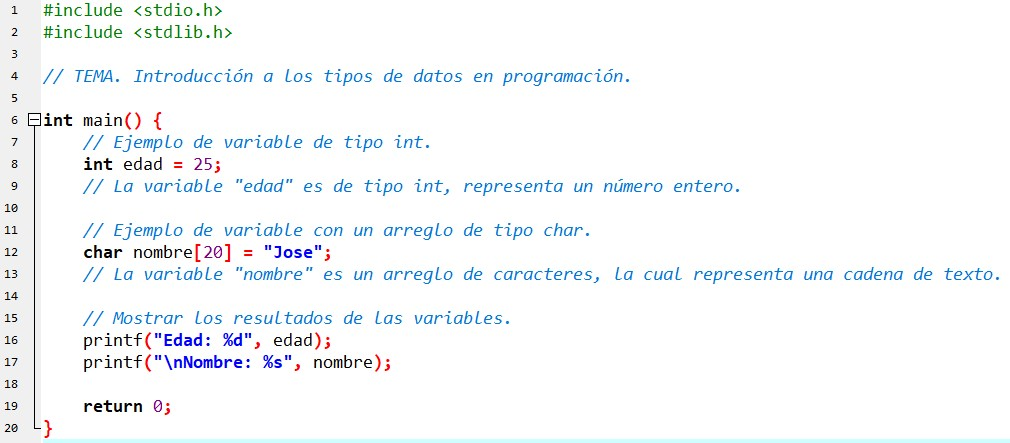
\includegraphics[width=0.9\textwidth]{codigo_tipos_datos.jpg}
    \caption{Programa en lenguaje C que ejemplifica el uso de tipos de datos y variables. Fuente: Elaboración propia.}
    \label{fig:codigo_tipos_datos}
\end{figure}

\begin{figure}[H]
    \centering
    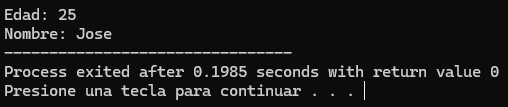
\includegraphics[width=0.5\textwidth]{resultado_codigo_tipos_datos.jpg}
    \caption{Salida del programa mostrado en la Figura \ref{fig:codigo_tipos_datos}. Fuente: Elaboración propia.}
    \label{fig:salida_codigo_tipos_datos}
\end{figure}


También es preciso señalar que, en C, los tipos de datos se clasifican en dos grandes grupos: primitivos (o básicos) y derivados. Primero los que se denominan tipos de datos primitivos, que son aquellos que el compilador reconoce de forma nativa, constituyendo los elementos fundamentales sobre los cuales se construyen los programas. Estos permiten representar información básica dentro de un sistema, facilitando su almacenamiento y manipulación de manera eficiente.

Los tipos de datos primitivos se clasifican a su vez en tres categorías según la naturaleza de la información que almacenan. Los tipos enteros están diseñados para representar números sin parte decimal e incluyen variantes como \texttt{char}, \texttt{int}, \texttt{short}, \texttt{long} y \texttt{long long}, así como el tipo \texttt{enum} para definir conjuntos de constantes. Por otro lado, los tipos reales permiten manejar valores con parte fraccionaria, como \texttt{float}, \texttt{double} y \texttt{long double}, dependiendo de la precisión requerida. Finalmente, los tipos lógicos se representan tradicionalmente mediante valores enteros, donde el valor \texttt{0} indica falso y cualquier valor distinto de cero indica verdadero \cite{frem_ref3}.

En segundo lugar, a diferencia de los tipos de datos primitivos, los tipos derivados se construyen a partir de la combinación o extensión de estos, lo que permite representar estructuras de información más complejas y manejar la memoria de manera más flexible dentro de un programa.
Entre los principales tipos derivados se encuentran los arreglos, que son colecciones de datos del mismo tipo almacenados de forma contigua en memoria; las estructuras y uniones, que permiten agrupar variables de distintos tipos bajo un mismo nombre; los punteros, que almacenan direcciones de memoria y facilitan un control más directo sobre los recursos del sistema; y las funciones, que, además de representar bloques de código reutilizables, también se consideran tipos derivados debido a que devuelven valores de un tipo específico \cite{frem_ref3}.

% ------------------------------------------
% 2.3  Tipos de enteros
% ------------------------------------------
\subsection{Tipos de enteros}

El tipo de dato más común en programación es el entero o \texttt{int}, el cual es ideal para manejar valores numéricos. Por lo general, estos se almacenan internamente utilizando 2 bytes (16 bits). En la Tabla~\ref{tab:enteros} se detallan los tipos de enteros fundamentales, especificando sus rangos de valores y el tamaño en memoria que ocupan según el equipo utilizado. Incluso, existen modificadores como \texttt{unsigned}, \texttt{short} e \texttt{int} que permiten ajustar el rango de estos números. En cuanto a su escritura, el sistema decimal corresponde a la base 10, como en los valores 100 o 450; para valores sin signo se añade el sufijo \texttt{U}, por ejemplo, 40000U. El sistema octal, de base 8, se utiliza frecuentemente en sistemas operativos y sus números comienzan con un 0, como en 0377. Por su parte, el sistema hexadecimal, de base 16, emplea el prefijo \texttt{0x} seguido de dígitos o letras de la A a la F, como en 0xFF16.

Cuando los tipos básicos no son suficientes para representar cifras muy grandes, se recurre a los enteros de tipo \texttt{long}. Existen variantes de este tipo que requieren 4 bytes (32 bits) de almacenamiento. Algunos ejemplos de declaración son \texttt{long medida\_milimetros;} y \texttt{unsigned long distancia\_media;}. Para asegurar que el compilador interprete una constante como un tipo largo, se debe agregar el sufijo \texttt{L} al final del número, como en la expresión \texttt{long numeros\_grandes = 40000L;} \cite{frem_ref2}.

\begin{table}[H]
    \centering
    \begin{tabular}{|p{3cm}|p{7cm}|}
        \hline
        \textbf{Tipo C} & \textbf{Rango de valores} \\
        \hline
        
        int & $-32,768 \dots +32,767$ \\
        \hline

        unsigned int & $0 \dots 65,535$ \\
        \hline

        short int & $-128 \dots +127$ \\
        \hline

        long & $-2,147,483,648 \dots 2,147,483,647$ \\
        \hline

        unsigned long & $0 \dots +4,294,967,295$ \\
        \hline

    \end{tabular}
    \caption{Tipos de datos enteros. Fuente: Elaboración propia con base en \cite{frem_ref2}.}
    \label{tab:enteros}
\end{table}

El programa presentado a continuación muestra el uso de diferentes tipos de datos enteros en lenguaje C, incluyendo \texttt{int}, \texttt{unsigned int}, \texttt{short int}, \texttt{long} y \texttt{unsigned long}. Cada variable es declarada con un valor dentro de su rango permitido y posteriormente se imprime en pantalla utilizando la función \texttt{printf}, empleando los especificadores de formato adecuados para cada tipo. En la Figura \ref{fig:codigo_enteros} se muestra el código fuente del programa, donde se observan las declaraciones y el uso de cada tipo de dato, mientras que en la Figura \ref{fig:salida_codigo_enteros} se presenta el resultado de la ejecución, evidenciando cómo se imprimen correctamente los valores asignados.

\begin{figure}[H]
    \centering
    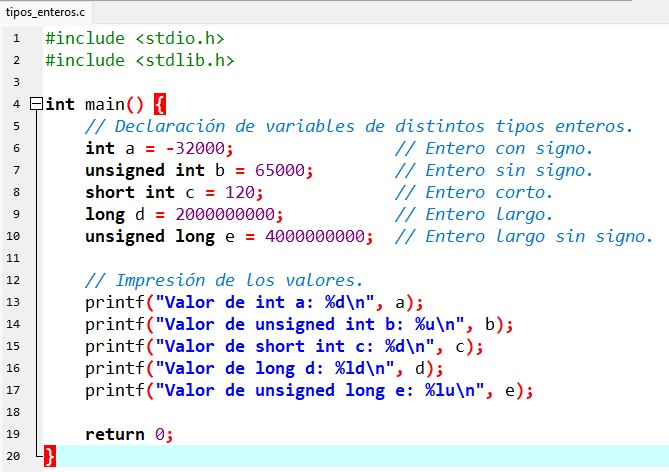
\includegraphics[width=0.6\textwidth]{codigo_enteros.jpg}
    \caption{Programa en lenguaje C que ejemplifica el uso de los tipos de enteros. Fuente: Elaboración propia.}
    \label{fig:codigo_enteros}
\end{figure}

\begin{figure}[H]
    \centering
    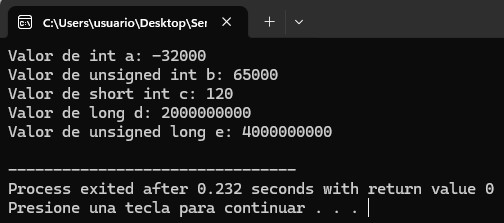
\includegraphics[width=0.5\textwidth]{resultado_codigo_enteros.jpg}
    \caption{Salida del programa mostrado en la Figura \ref{fig:codigo_enteros}. Fuente: Elaboración propia.}
    \label{fig:salida_codigo_enteros}
\end{figure}

% ------------------------------------------
% 2.4  Tipos de coma flotante
% ------------------------------------------
\subsection{Tipos de coma flotante}

Los tipos de datos de punto flotante permiten representar valores numéricos reales, es decir, aquellos que incluyen una parte decimal. Estos datos son útiles tanto para expresar cantidades con precisión, como 3.14159, como para manejar números de gran magnitud mediante notación científica, por ejemplo, $1.85 \times 10^{15}$. La forma de declarar variables de tipo flotante es similar a la utilizada para variables enteras, como se muestra en la Tabla~\ref{tab:declaracion_flotantes}.

\begin{table}[H]
    \centering
    \begin{tabular}{|p{5cm}|p{8cm}|}
        \hline
        \textbf{Caso} & \textbf{Ejemplo en C} \\
        \hline
        Declaración de una variable & \texttt{float valor;} \\
        \hline
        Declaración de varias variables & \texttt{float valor1, valor2;} \\
        \hline
        Declaración con inicialización & \texttt{float valor = 99.99;} \\
        \hline
    \end{tabular}
    \caption{Ejemplos comunes de declaración de variables de tipo flotante. Fuente: Elaboración propia.}
    \label{tab:declaracion_flotantes}
\end{table}

El lenguaje C admite diferentes formatos de números de punto flotante, como \texttt{float}, \texttt{double} y \texttt{long double}, los cuales varían en precisión y en el espacio de memoria requerido. Generalmente, el tipo \texttt{float} ocupa 4 bytes, \texttt{double} utiliza 8 bytes, y \texttt{long double} puede requerir mayor cantidad de memoria dependiendo del compilador \cite{frem_ref2}.

\begin{table}[H]
    \centering
    \begin{tabular}{|p{3cm}|p{5cm}|p{3cm}|}
        \hline
        \textbf{Tipo C} & \textbf{Rango de valores} & \textbf{Precisión} \\
        \hline

        float & $3.4 \times 10^{-38} \dots 3.4 \times 10^{38}$ & 7 dígitos \\
        \hline

        double & $1.7 \times 10^{-308} \dots 1.7 \times 10^{308}$ & 15 dígitos \\
        \hline

        long double & $3.4 \times 10^{-4932} \dots 1.1 \times 10^{4932}$ & 19 dígitos \\
        \hline

    \end{tabular}
    \caption{Tipos de datos en coma flotante. Fuente: \cite{frem_ref2}.}
    \label{tab:flotantes}
\end{table}

El programa muestra el uso de los tipos de datos \texttt{float}, \texttt{double} y \texttt{long double} en C, así como una comparación básica de su precisión y tamaño en memoria. En la Figura~\ref{fig:codigo_flotantes} se presenta el código, donde se incluye la directiva \texttt{\#define \_\_USE\_MINGW\_ANSI\_STDIO 1}, la cual se utiliza en compiladores como MinGW para asegurar que funciones como \texttt{printf} manejen correctamente formatos avanzados (por ejemplo, \texttt{\%Lf} para \texttt{long double}). Posteriormente, se declaran variables de cada tipo, se imprimen sus valores y se utiliza el operador \texttt{sizeof} para conocer cuántos bytes ocupa cada uno. En la Figura~\ref{fig:salida_codigo_flotantes} se observa el resultado de la ejecución, donde se puede notar que, aunque los valores impresos son similares, los tamaños en memoria son diferentes, siendo \texttt{float} el de menor tamaño y \texttt{long double} el de mayor, lo que está directamente relacionado con la precisión que cada tipo puede manejar.

\begin{figure}[H]
    \centering
    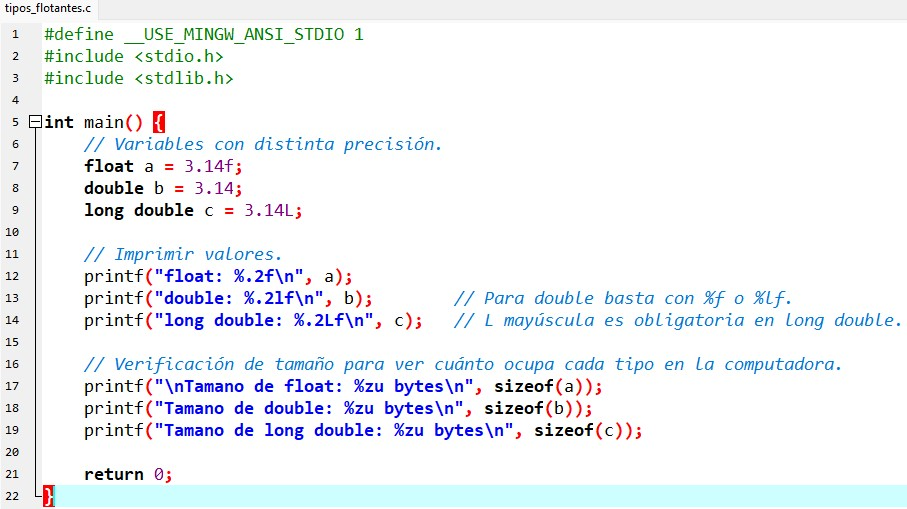
\includegraphics[width=0.8\textwidth]{codigo_flotantes.jpg}
    \caption{Programa en lenguaje C que ejemplifica el uso de los tipos de flotantes. Fuente: Elaboración propia.}
    \label{fig:codigo_flotantes}
\end{figure}

\begin{figure}[H]
    \centering
    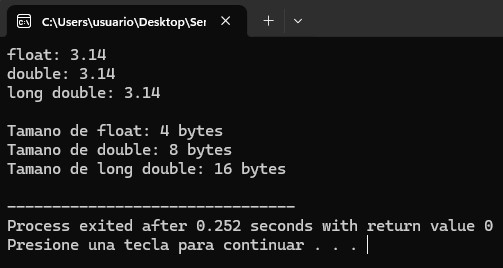
\includegraphics[width=0.5\textwidth]{resultado_codigo_flotantes.jpg}
    \caption{Salida del programa mostrado en la Figura \ref{fig:codigo_flotantes}. Fuente: Elaboración propia.}
    \label{fig:salida_codigo_flotantes}
\end{figure}

% ------------------------------------------
% 2.5  Caracteres
% ------------------------------------------
\subsection{Caracteres}

En el lenguaje C, un carácter se entiende como la unidad mínima dentro de un conjunto de símbolos definido, siendo el estándar ASCII uno de los más utilizados en los sistemas de cómputo. Para representar este tipo de información se utiliza el tipo de dato \texttt{char}, el cual también puede formar parte de arreglos para construir cadenas de caracteres. Aunque los caracteres se interpretan visualmente como letras o símbolos, internamente se manejan como valores numéricos; por ejemplo, el carácter \texttt{'A'} equivale al valor 65 en código ASCII. Esta representación permite realizar operaciones aritméticas sobre ellos, lo que facilita procesos como la conversión entre letras mayúsculas y minúsculas mediante la suma o resta de 32 unidades.

El tipo \texttt{char} con signo generalmente cubre un rango de $-128$ a $127$, mientras que la variante \texttt{unsigned char} permite representar valores en el intervalo de $0$ a $255$, abarcando así todo el conjunto ASCII extendido. Dado que los caracteres forman parte de la familia de los enteros, es posible asignarlos a variables de tipo \texttt{int} para efectuar operaciones adicionales. Asimismo, el lenguaje C proporciona secuencias de escape para representar caracteres especiales que no pueden escribirse de forma directa, como \texttt{\textbackslash n} para indicar un salto de línea o \texttt{\textbackslash '} para representar una comilla simple. Estas secuencias se presentan en la Tabla~\ref{tab:caracteres_secuencia} \cite{frem_ref2}.

\begin{table}[H]
    \centering
    \begin{tabular}{|p{3cm}|p{5cm}|p{4cm}|}
        \hline
        \textbf{Código de escape} & \textbf{Significado} & \textbf{Código ASCII (Decimal)} \\
        \hline

        \texttt{\textbackslash n} & nueva línea & 10 \\ \hline
        \texttt{\textbackslash r} & retorno de carro & 13 \\ \hline
        \texttt{\textbackslash t} & tabulación & 9 \\ \hline
        \texttt{\textbackslash v} & tabulación vertical & 11 \\ \hline
        \texttt{\textbackslash a} & alerta (pitido sonoro) & 7 \\ \hline
        \texttt{\textbackslash b} & retroceso de espacio & 8 \\ \hline
        \texttt{\textbackslash f} & avance de página & 12 \\ \hline
        \texttt{\textbackslash \textbackslash} & barra inclinada inversa & 92 \\ \hline
        \texttt{\textbackslash '} & comilla simple & 39 \\ \hline
        \texttt{\textbackslash "} & doble comilla & 34 \\ \hline
        \texttt{\textbackslash ?} & signo de interrogación & 63 \\ \hline

    \end{tabular}
    \caption{Caracteres secuencias (códigos) de escape. Fuente: \cite{frem_ref2}.}
    \label{tab:caracteres_secuencia}
\end{table}

A continuación se presenta un ejemplo que ilustra el uso del tipo de dato \texttt{char} en el lenguaje C, así como su relación con la aritmética de enteros y algunas secuencias de escape comunes. En la Figura~\ref{fig:codigo_char} se muestra el código del programa, donde se declara una variable de tipo carácter y se realiza una operación aritmética simple al sumarle una unidad, lo que permite obtener el siguiente carácter según la tabla ASCII. Además, se imprimen tanto los caracteres como sus valores numéricos equivalentes, evidenciando que internamente se manejan como enteros. También se incluyen ejemplos de secuencias de escape como \texttt{\textbackslash n}, \texttt{\textbackslash t} y el uso de comillas, las cuales permiten dar formato a la salida en pantalla. En la Figura~\ref{fig:salida_codigo_char} se presenta la salida obtenida al ejecutar el programa, donde se observan los cambios en los caracteres, sus valores ASCII y el efecto de las secuencias de escape en el formato del texto.

\begin{figure}[H]
    \centering
    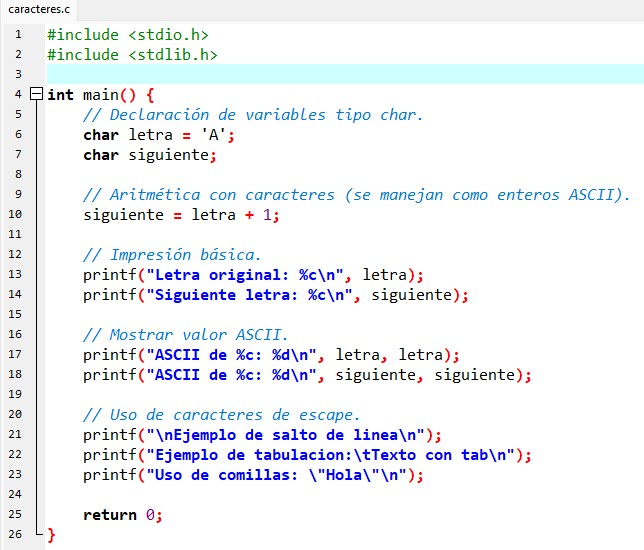
\includegraphics[width=0.7\textwidth]{codigo_caracteres.jpg}
    \caption{Programa en lenguaje C que ejemplifica el uso del tipo char. Fuente: Elaboración propia.}
    \label{fig:codigo_char}
\end{figure}

\begin{figure}[H]
    \centering
    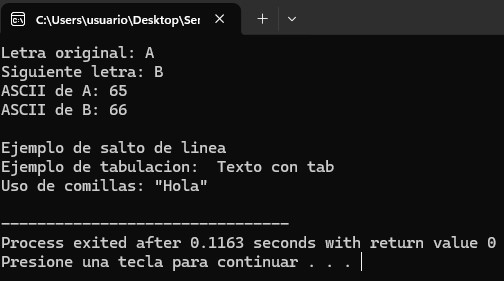
\includegraphics[width=0.5\textwidth]{resultado_codigo_caracteres.jpg}
    \caption{Salida del programa mostrado en la Figura \ref{fig:codigo_char}. Fuente: Elaboración propia.}
    \label{fig:salida_codigo_char}
\end{figure}

% ------------------------------------------
% 2.6  Tipo de dato lógico
% ------------------------------------------
\subsection{Tipo de dato lógico}

Según \cite{frem_ref2}, los compiladores de C que se ajustan al estándar ANSI no contemplan de manera nativa un tipo de dato lógico con valores explícitos como \textit{true} y \textit{false}. En su lugar, este lenguaje emplea el tipo entero para representar condiciones lógicas dentro de estructuras de control como \texttt{if} y \texttt{while}. En este contexto, el valor 0 se interpreta como falso, mientras que cualquier valor distinto de cero se considera verdadero. Esto permite construir expresiones lógicas sin requerir un tipo booleano específico, a diferencia de otros lenguajes que sí lo incorporan directamente. Así, cualquier expresión que evalúe a 0 se asocia con falso, mientras que cualquier otro valor entero representa verdadero. Para ejemplificarlo, la evaluación e impresión de valores lógicos en C se resumen en la Tabla~\ref{tab:ejemplos_tipo_logico}.

\begin{table}[H]
    \centering
    \begin{tabular}{|p{5.5cm}|p{7.5cm}|}
        \hline
        \textbf{Caso} & \textbf{Ejemplo en C} \\
        \hline
        Declaración de variables de control lógico & \texttt{int bisiesto; bisiesto = 1; int encontrado, bandera;} \\
        \hline
        Estructura condicional & \texttt{if (encontrado) ...} \\
        \hline
        Asignación de valor falso & \texttt{indicador = 0;} \\
        \hline
        Asignación por comparación relacional & \texttt{indicador = suma > 10;} \\
        \hline
        Tipo lógico definido por enumeración & \texttt{enum Boolean \{ FALSE, TRUE \};} \\
        \hline
        Impresión del valor lógico & \texttt{printf(\comillas{El valor de encontrado es \%d\textbackslash n}, encontrado);} \\
        \hline
        Salida cuando \texttt{encontrado = 0} & \texttt{El valor de encontrado es 0} \\
        \hline
    \end{tabular}
    \caption{Ejemplos de uso del tipo de dato lógico en lenguaje C. Fuente: Elaboración propia.}
    \label{tab:ejemplos_tipo_logico}
\end{table}

De esta forma, en C cualquier valor diferente de cero indica una condición verdadera, mientras que el valor cero representa una condición falsa.
El lenguaje también permite la creación de tipos definidos por el usuario mediante enumeraciones, donde se asignan valores enteros a identificadores simbólicos. Con esta declaración se establece un nuevo tipo denominado \texttt{Boolean}, que incluye las constantes \texttt{FALSE} y \texttt{TRUE} asociadas a valores enteros. Por lo general, las expresiones lógicas se utilizan en estructuras que controlan el flujo del programa. Aunque no suelen emplearse directamente como datos de entrada, sí pueden mostrarse como parte de la salida mediante la función \texttt{printf()}, como también se observa en la Tabla~\ref{tab:ejemplos_tipo_logico}.

Enseguida se presenta un programa que ejemplifica el manejo de valores lógicos en el lenguaje C mediante el uso de variables enteras y un tipo definido con \texttt{enum}. En la Figura~\ref{fig:codigo_bool} se observa el código, donde se evalúa una condición relacional cuyo resultado se almacena en una variable entera, tomando el valor de 1 si la condición es verdadera o 0 en caso contrario. Asimismo, se emplea un tipo enumerado para representar de manera más clara los valores lógicos, facilitando la lectura del programa. Estas variables son utilizadas dentro de estructuras condicionales para controlar el flujo de ejecución. En la Figura~\ref{fig:salida_codigo_bool} se muestra la salida del programa, en la cual se pueden apreciar los valores numéricos asociados a las condiciones evaluadas, así como los mensajes generados dependiendo del resultado de las mismas.

\begin{figure}[H]
    \centering
    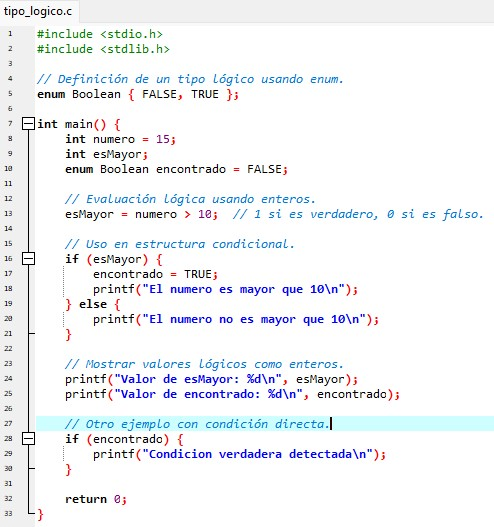
\includegraphics[width=0.6\textwidth]{codigo_tipo_logico.jpg}
    \caption{Programa en lenguaje C que ejemplifica el uso del tipo lógico. Fuente: Elaboración propia.}
    \label{fig:codigo_bool}
\end{figure}

\begin{figure}[H]
    \centering
    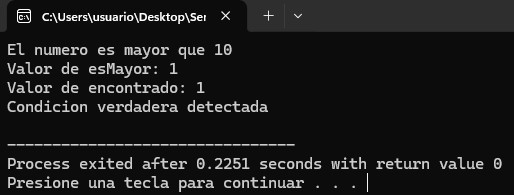
\includegraphics[width=0.5\textwidth]{resultado_codigo_tipo_logico.jpg}
    \caption{Salida del programa mostrado en la Figura \ref{fig:codigo_bool}. Fuente: Elaboración propia.}
    \label{fig:salida_codigo_bool}
\end{figure}

% ------------------------------------------
% 2.7  Arrays
% ------------------------------------------
\subsection{Arrays}

Un arreglo se define como una agrupación de elementos del mismo tipo de dato que se almacenan de manera contigua en la memoria. Para distinguir cada componente dentro de esta colección, se utiliza un número de orden denominado índice o subíndice. Al igual que cualquier otra variable, un arreglo debe declararse antes de ser utilizado en un programa. Para definirlo correctamente, es necesario especificar tres elementos fundamentales: el tipo de dato, que determina la clase de valores que almacenará, como \texttt{int}, \texttt{char} o \texttt{float}; el nombre, que funciona como el identificador único del arreglo; y el tamaño, que indica la cantidad máxima de elementos que la estructura puede contener. La sintaxis general para su declaración se escribe como \texttt{tipo nombre[tamaño];}, de manera que, por ejemplo, al declarar \texttt{int marks[10];} se reserva espacio para diez números enteros como se puede ver en la Figura \ref{fig:representacion_array}.

\begin{figure}[H]
    \centering
    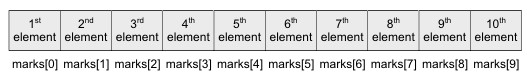
\includegraphics[width=0.8\textwidth]{representacion_array.jpg}
    \caption{Representación en memoria de un arreglo de 10 elementos \cite{frem_ref4}.}
    \label{fig:representacion_array}
\end{figure}

Además, para ilustrar cómo se pueden declarar diferentes tipos de arreglos y cómo se representan sus elementos de manera visual, en la Figura~\ref{fig:declaracion_arrays} se muestra un ejemplo gráfico de tres tipos de arreglos en C, cada uno con distintos tipos de datos. La imagen permite observar la estructura y distribución de los elementos dentro de cada arreglo, facilitando la comprensión de cómo se organizan en la memoria del programa \cite{frem_ref4}.

\begin{figure}[H]
    \centering
    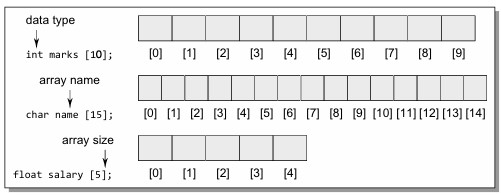
\includegraphics[width=0.6\textwidth]{declaracion_arrays.jpg}
    \caption{Declaración de arreglos de diferentes tipos de datos y tamaños \cite{frem_ref4}.}
    \label{fig:declaracion_arrays}
\end{figure}

Posteriormente, se presenta un programa que ejemplifica el uso de arreglos en el lenguaje C con distintos tipos de datos: enteros, flotantes y caracteres. En la Figura~\ref{fig:codigo_array} se muestra el código, donde se declaran e inicializan tres arreglos y se recorren mediante ciclos \texttt{for} para acceder a sus elementos. En el caso del arreglo de enteros, se realiza la suma de sus valores, mientras que con el arreglo de flotantes se calcula el promedio de los datos almacenados. Por otra parte, el arreglo de caracteres se utiliza como una cadena de texto, recorriéndose hasta encontrar el carácter nulo que indica el final de la misma. En la Figura~\ref{fig:salida_codigo_array} se presenta la salida del programa, donde se observan los valores almacenados en cada arreglo, así como los resultados de las operaciones realizadas, lo que permite comprender la forma en que se manipulan diferentes tipos de datos mediante estructuras de tipo arreglo.

\begin{figure}[H]
    \centering
    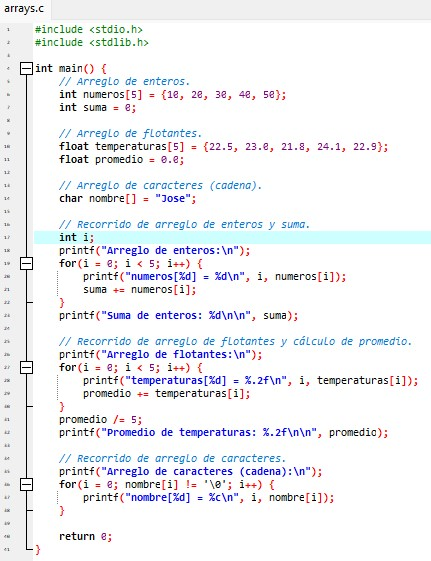
\includegraphics[width=0.6\textwidth]{codigo_arrays.jpg}
    \caption{Programa en lenguaje C que ejemplifica el uso de arreglos. Fuente: Elaboración propia.}
    \label{fig:codigo_array}
\end{figure}

\begin{figure}[H]
    \centering
    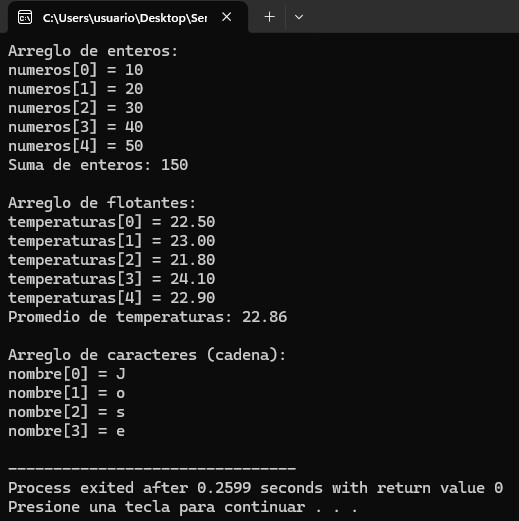
\includegraphics[width=0.5\textwidth]{resultado_codigo_arrays.jpg}
    \caption{Salida del programa mostrado en la Figura \ref{fig:codigo_array}. Fuente: Elaboración propia.}
    \label{fig:salida_codigo_array}
\end{figure}

% ------------------------------------------
% 2.8  Punteros
% ------------------------------------------
\subsection{Punteros}

En el lenguaje C, los punteros constituyen una de las herramientas más importantes para trabajar con la memoria de forma directa. A diferencia de una variable común, que almacena un valor, un puntero almacena la dirección de memoria donde se encuentra dicho valor. Gracias a ello, es posible acceder, modificar y compartir datos entre distintas partes del programa con mayor eficiencia, especialmente en tareas como el manejo de arreglos, el paso de parámetros por referencia y la asignación dinámica de memoria.

Comprender los punteros también permite interpretar mejor cómo se relacionan las variables con su ubicación física en memoria durante la ejecución. Por esta razón, antes de profundizar en su sintaxis y uso práctico, resulta necesario revisar primero el concepto de dirección de memoria y la forma en que C permite consultarla e imprimirla.

\subsubsection{Direcciones de memoria}

De acuerdo con \cite{frem_ref2} cuando se declara una variable en C, se le asocian tres características principales: su nombre, su tipo de dato y la dirección de memoria donde se almacena. El valor de una variable se obtiene utilizando directamente su nombre, mientras que su dirección de memoria se consulta con el operador \texttt{\&}; ambos casos se resumen en la Tabla~\ref{tab:direccion_memoria_c}.

\begin{table}[H]
    \centering
    \begin{tabular}{|p{5.5cm}|p{7.5cm}|}
        \hline
        \textbf{Caso} & \textbf{Ejemplo en C} \\
        \hline
        Mostrar el valor de una variable & \texttt{printf("\%d", n);} \\
        \hline
        Mostrar la dirección de memoria de una variable & \texttt{printf("\%p", \&n);} \\
        \hline
    \end{tabular}
    \caption{Ejemplos para imprimir el valor y la dirección de memoria de una variable en C. Fuente: Elaboración propia.}
    \label{tab:direccion_memoria_c}
\end{table}

A continuación, en la Figura~\ref{fig:codigo_direccion}, se presenta un programa de ejemplo que permite observar cómo imprimir tanto el valor de una variable como su dirección de memoria. En la Figura~\ref{fig:resultado_direccion} se muestran los resultados obtenidos. En este caso, el especificador de formato \texttt{\%d} se utiliza para imprimir el valor entero de la variable, mientras que \texttt{\%p} permite mostrar la dirección de memoria en formato hexadecimal. Cabe destacar que este valor puede variar dependiendo de la computadora de cada usuario y generalmente se presenta con el prefijo \texttt{0x}.

\begin{figure}[H]
    \centering
    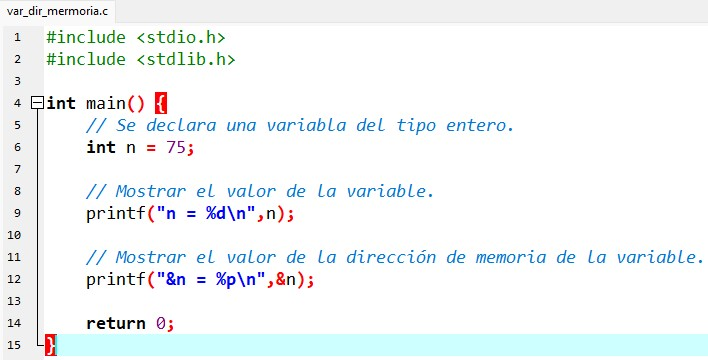
\includegraphics[width=0.7\textwidth]{codigo_memoria.jpg}
    \caption{Programa en lenguaje C que ejemplifica la forma para obtener el valor y la dirección de una variable. Fuente: Elaboración propia con base en \cite{frem_ref2}.}
    \label{fig:codigo_direccion}
\end{figure}

\begin{figure}[H]
    \centering
    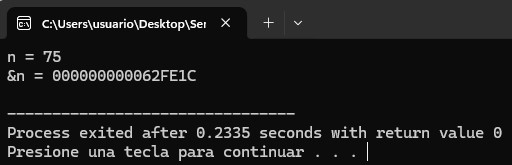
\includegraphics[width=0.5\textwidth]{resultado_codigo_memoria.jpg}
    \caption{Salida del programa mostrado en la Figura \ref{fig:codigo_direccion}. Fuente: Elaboración propia.}
    \label{fig:resultado_direccion}
\end{figure}

\subsubsection{Apuntadores}

Una vez comprendida la noción de dirección de memoria, el siguiente paso es estudiar los apuntadores, que permiten gestionar esas direcciones de manera explícita dentro del programa. Un apuntador se define esencialmente como una variable cuyo propósito no es guardar un dato común, sino registrar la dirección de memoria de otra variable. Este concepto es comparable a elementos cotidianos como una dirección postal o un número telefónico, ya que ambos funcionan como indicadores que señalan dónde localizar un destino o una persona específica. En programación, el apuntador actúa como ese mapa que le indica al software exactamente en qué posición de la memoria se encuentran los datos asociados a una variable determinada.

Desde una perspectiva técnica, el apuntador opera bajo la premisa de ser una variable que contiene una dirección apuntando a una posición de memoria ajena, permitiendo que el sistema recupere la información depositada en ese punto exacto. En resumen, cualquier variable que cumpla la función de almacenar una dirección de memoria se denomina formalmente apuntador, sirviendo como un enlace directo hacia la ubicación física de los datos en el hardware \cite{frem_ref2}.

La imagen de la Figura \ref{fig:apuntadores} ilustra de forma gráfica cómo un apuntador almacena una dirección física de la memoria en lugar de un dato convencional. En el diagrama, se observa que la variable p (ubicada en la dirección 1000) contiene el valor 100, el cual corresponde precisamente a la dirección donde se encuentra guardada la variable alfa; de esta manera, al utilizar el operador de indirección (*p), el sistema puede acceder directamente al contenido de esa posición, que en este caso es el carácter 'A'.

\begin{figure}[H]
    \centering
    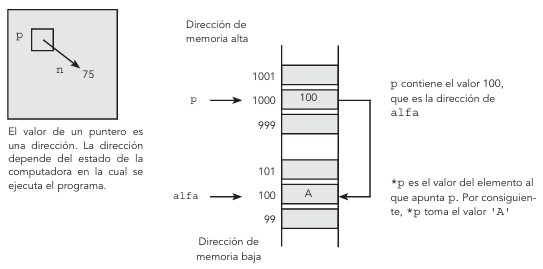
\includegraphics[width=0.6\textwidth]{apuntadores.jpg}
    \caption{Relaciones entre *p y el valor de p (dirección de alfa) \cite{frem_ref2}.}
    \label{fig:apuntadores}
\end{figure}

El programa en C de la Figura \ref{fig:codigo_apuntador} pone en práctica el concepto visual al declarar un entero n con el valor 75 y un apuntador p que vincula su dirección mediante el operador \&n. A través de las funciones de impresión, en la Figura \ref{fig:resultado_apuntador}, el código demuestra la relación entre la variable original y el apuntador, permitiendo visualizar tanto el valor numérico de n como las direcciones de memoria específicas que el compilador ha asignado para cada variable durante la ejecución.

\begin{figure}[H]
    \centering
    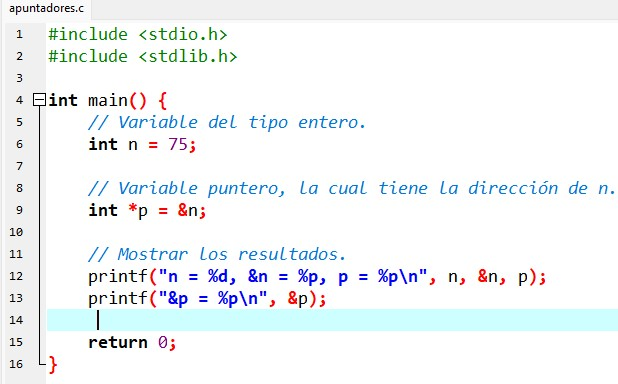
\includegraphics[width=0.6\textwidth]{codigo_apuntadores.jpg}
    \caption{Programa en lenguaje C que ejemplifica el uso de apuntadores. Fuente: Elaboración propia con base en \cite{frem_ref2}.}
    \label{fig:codigo_apuntador}
\end{figure}

\begin{figure}[H]
    \centering
    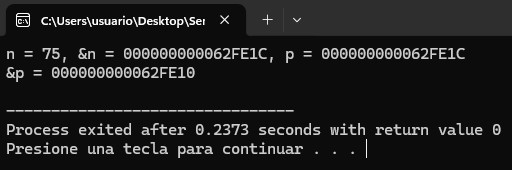
\includegraphics[width=0.5\textwidth]{resultado_codigo_apuntadores.jpg}
    \caption{Salida del programa mostrado en la Figura \ref{fig:codigo_apuntador}. Fuente: Elaboración propia.}
    \label{fig:resultado_apuntador}
\end{figure}

% ------------------------------------------
% 2.9  Funciones
% ------------------------------------------
\subsection{Funciones}

El lenguaje C permite estructurar los programas en segmentos independientes conocidos como funciones, las cuales facilitan la organización y reutilización del código. Cada función está diseñada para realizar una tarea específica, lo que contribuye a que el programa sea más claro, modular y fácil de mantener. En este sentido, el código de una función se mantiene separado del resto, evitando dependencias innecesarias entre diferentes partes del programa.

Cada función se comunica con el entorno exterior mediante una interfaz definida por su nombre, parámetros y valor de retorno. Esto permite enviar información hacia la función y recibir resultados después de su ejecución. En la Figura~\ref{fig:funciones_1} se ilustra un ejemplo donde la función principal \texttt{main()} realiza una llamada a otra función, transfiriendo el control de ejecución. A esta función invocada se le conoce como función llamada, mientras que \texttt{main()} actúa como función llamadora. Una vez que la función llamada finaliza su ejecución, el control regresa al punto desde donde fue invocada.

\begin{figure}[H]
    \centering
    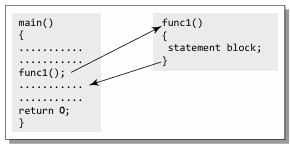
\includegraphics[width=0.4\textwidth]{funcion_1.jpg}
    \caption{Función principal (main) y llamada a la función (func1) \cite{frem_ref4}.}
    \label{fig:funciones_1}
\end{figure}

Además, una función puede ser utilizada múltiples veces dentro de un programa, incluso dentro de estructuras repetitivas como ciclos \texttt{for}, \texttt{while} o \texttt{do-while}, lo que permite ejecutar la misma tarea varias veces sin necesidad de repetir código. Esto mejora la eficiencia y reduce errores.

No solo la función principal puede invocar otras funciones, sino que cualquier función puede llamar a otra, generando una estructura más compleja de ejecución. En la Figura~\ref{fig:funciones_2} se muestra un ejemplo donde varias funciones se llaman entre sí de manera encadenada, permitiendo dividir el problema en subproblemas más pequeños y manejables \cite{frem_ref4}.

\begin{figure}[H]
    \centering
    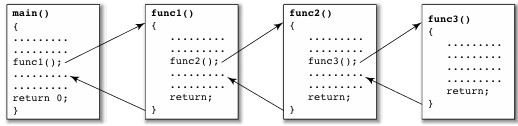
\includegraphics[width=0.6\textwidth]{funcion_2.jpg}
    \caption{Llamadas a diferentes funciones \cite{frem_ref4}.}
    \label{fig:funciones_2}
\end{figure}

En esta sección se presenta un ejemplo que ilustra el uso de funciones en el lenguaje C, considerando tanto funciones con valor de retorno como aquellas que no lo poseen. En la Figura~\ref{fig:codigo_funciones} se muestra el programa, donde se define una función sin retorno que imprime un mensaje en pantalla, así como otra función que recibe parámetros, realiza una operación y devuelve un resultado. Ambas funciones son invocadas desde la función principal \texttt{main()}, lo que permite observar la transferencia de control y el uso de valores de retorno. En la Figura~\ref{fig:resultado_funciones} se presenta la salida del programa, donde se visualiza el mensaje generado por la función sin retorno y el resultado de la operación realizada por la función con retorno.

\begin{figure}[H]
    \centering
    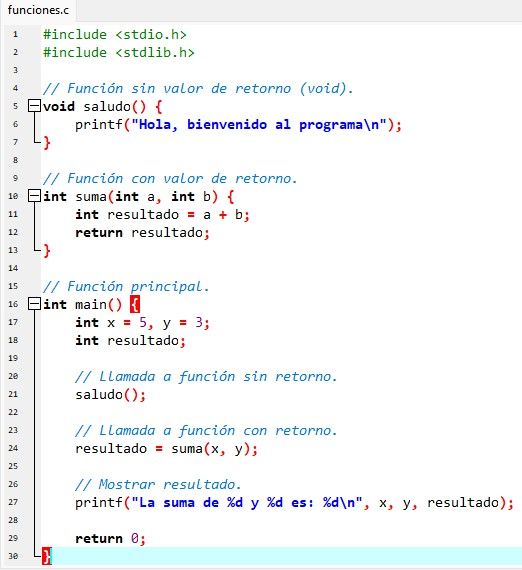
\includegraphics[width=0.6\textwidth]{codigo_funciones.jpg}
    \caption{Programa en lenguaje C que ejemplifica el uso de funciones. Fuente: Elaboración propia.}
    \label{fig:codigo_funciones}
\end{figure}

\begin{figure}[H]
    \centering
    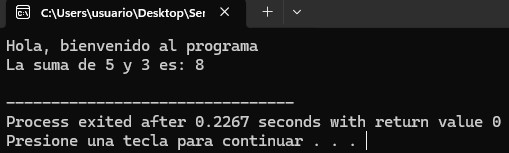
\includegraphics[width=0.5\textwidth]{resultado_codigo_funciones.jpg}
    \caption{Salida del programa mostrado en la Figura \ref{fig:codigo_funciones}. Fuente: Elaboración propia.}
    \label{fig:resultado_funciones}
\end{figure}

% ------------------------------------------
% 2.10  Estructuras
% ------------------------------------------
\subsection{Estructuras}

De acuerdo con \cite{frem_ref5}, una estructura en el lenguaje C es un tipo de dato compuesto que permite agrupar un conjunto finito de elementos que pueden ser de distintos tipos. Este mecanismo resulta útil para representar información más compleja, especialmente cuando se requiere trabajar con datos organizados en forma de registros.

En términos generales, una estructura se define como una colección de variables relacionadas entre sí, pero que pueden pertenecer a diferentes tipos de datos, todas agrupadas bajo un mismo identificador para facilitar su manipulación. Su uso es frecuente en aplicaciones como bases de datos, donde se manejan conjuntos de información organizados en registros. La sintaxis principal para definir, declarar y manipular estructuras en C se resume en la Tabla~\ref{tab:estructuras_sintaxis_c}.

\begin{table}[H]
    \centering
    \begin{tabular}{|p{4.2cm}|p{5.6cm}|p{3.2cm}|}
        \hline
        \textbf{Caso} & \textbf{Ejemplo en C} & \textbf{Diferencia clave / uso} \\
        \hline
        Definición básica de una estructura & \texttt{struct Alumno \{ char nombre[30]; int edad; float promedio; \};} & Crea un nuevo tipo compuesto. \\
        \hline
        Definir estructura y declarar variables después & \texttt{struct Trabajador \{ ... \}; struct Trabajador fijo, temporal;} & Permite declarar más variables del mismo tipo en otras partes. \\
        \hline
        Definir estructura y declarar variables al mismo tiempo & \texttt{struct Trabajador \{ ... \} fijo, temporal;} & Es más compacto, pero menos flexible para reutilizar. \\
        \hline
        Acceso a campos mediante operador punto & \texttt{alumno.promedio;} & Se usa cuando se trabaja con una variable estructura (no puntero). \\
        \hline
        Asignación a un campo específico & \texttt{temporal.edad = 25;} & Modifica solo un miembro de la estructura. \\
        \hline
        Asignación entre estructuras del mismo tipo & \texttt{fijo = temporal;} & Copia todos los campos; ambas variables deben ser del mismo tipo. \\
        \hline
        Inicialización al declarar & \texttt{struct Trabajador fijo = \{"Pedro", "Hernández", 32, "gerente"\};} & Debe respetar el orden de los campos definidos. \\
        \hline
        Inicialización de campos tipo arreglo & \texttt{struct Notas alumno = \{\comillas{Carlos}, \{8,7,9,6,10\}\};} & Los arreglos se inicializan con llaves internas. \\
        \hline
    \end{tabular}
    \caption{Sintaxis, ejemplos y diferencias de uso de estructuras en C. Fuente: Elaboración propia.}
    \label{tab:estructuras_sintaxis_c}
\end{table}

En esta definición, \texttt{tipo\_estructura} corresponde al nombre del nuevo tipo de dato creado, mientras que \texttt{tipo\_variable} y \texttt{nombre\_variable} representan los tipos y nombres de los campos que conforman la estructura. En general, puede definirse primero la estructura y declarar variables después, o bien realizar ambas acciones en una sola sentencia, como se observa en la Tabla~\ref{tab:estructuras_sintaxis_c}. La estructura debe declararse antes de ser utilizada, normalmente antes de la función \texttt{main}. El acceso a los campos se realiza con el operador punto y, una vez definidas, las estructuras del mismo tipo pueden asignarse entre sí. Asimismo, es posible inicializarlas desde su declaración, incluyendo arreglos entre llaves cuando un campo corresponde a este tipo de dato, tal como también se muestra en la Tabla~\ref{tab:estructuras_sintaxis_c}.

Además de esto en la Figura~\ref{fig:codigo_struct} se muestra el programa, donde se define una estructura denominada \texttt{Alumno}, la cual agrupa diferentes tipos de datos relacionados, como nombre, edad y promedio. Posteriormente, se declara un arreglo de estructuras que permite almacenar la información de varios alumnos, funcionando como un conjunto de registros. Los datos son capturados mediante entrada estándar y posteriormente mostrados en pantalla utilizando un ciclo. En la Figura~\ref{fig:resultado_struct} se presenta la salida del programa, donde se visualiza la información almacenada en cada registro, lo que permite comprender cómo las estructuras facilitan la organización de datos relacionados en un solo elemento.

\begin{figure}[H]
    \centering
    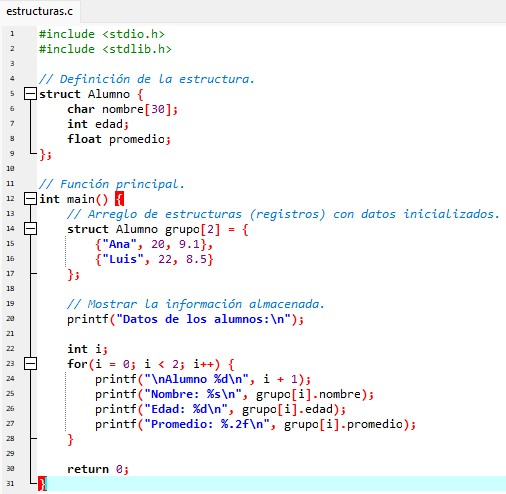
\includegraphics[width=0.6\textwidth]{codigo_estructuras.jpg}
    \caption{Programa en lenguaje C que ejemplifica el uso de funciones. Fuente: Elaboración propia.}
    \label{fig:codigo_struct}
\end{figure}

\begin{figure}[H]
    \centering
    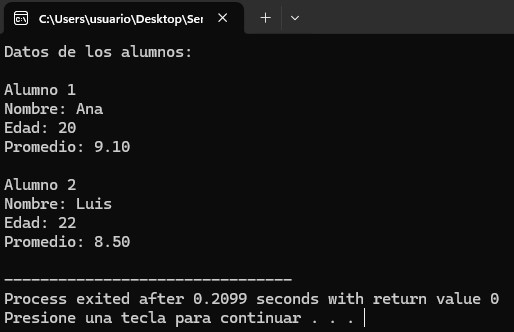
\includegraphics[width=0.5\textwidth]{resultado_codigo_estructuras.jpg}
    \caption{Salida del programa mostrado en la Figura \ref{fig:codigo_struct}. Fuente: Elaboración propia.}
    \label{fig:resultado_struct}
\end{figure}

% ==========================================
% SECCIÓN 2: PROCESOS
% ==========================================
% TIP: Esta sección describe qué es un proceso, los tipos de procesos y cómo se utilizan en C, es decir, cómo se crean y gestionan, y su importancia en la programación concurrente.
%
% TIP: Las rutas de imágenes son relativas a main.tex.
%
% ==========================================
\section{Procesos en C}
\label{sec:procesos}

% ------------------------------------------
% Responsable: Luna Gonzales Gabriel Alexis
% ------------------------------------------

% TODO (Gabriel): Describir qué es un proceso, los tipos de procesos (padre, hijo, zombi, huérfano) y cómo se utilizan en C, es decir, cómo se crean y gestionan, y su importancia en la programación concurrente.
% TODO (Gabriel): Incluir ejemplos de código para cada tipo de proceso.
% ==========================================
% SECCIÓN 3: ARCHIVOS
% ==========================================
% TIP: Esta sección describe cómo se manejan los archivos en C, incluyendo la lectura y escritura de archivos, los modos de apertura, y ejemplos prácticos de uso.
%
% TIP: Las rutas de imágenes son relativas a main.tex.
%
% ==========================================
\section{Archivos en C}
\label{sec:archivos}

% ------------------------------------------
% Responsable: Cristian Delgado Lucero Isaac
% ------------------------------------------

% TODO (Cristian): Describir cómo se manejan los archivos en C, incluyendo la lectura y escritura de archivos, los modos de apertura, y ejemplos prácticos de uso.
% TODO (Cristian): Incluir ejemplos de código para cada tipo de archivo.

La evolución de la informática hacia arquitecturas de procesamiento paralelo ha exigido una redefinición constante de las abstracciones que permiten a los programas interactuar con el almacenamiento persistente. En el contexto de la programación de sistemas en lenguaje C y el desarrollo de aplicaciones paralelas, el concepto de "archivo" trasciende la mera secuencia de bytes en un disco para convertirse en un recurso compartido cuya gestión requiere una sincronización meticulosa, una comprensión de la herencia de recursos entre procesos y una optimización profunda de los mecanismos de transferencia de datos.

\subsection{Definiciones Fundamentales}

Para comprender la manipulación de datos en cómputo paralelo, es necesario definir las entidades básicas con las que interactúa el sistema operativo y el programador. Estas entidades constituyen los bloques fundamentales sobre los cuales se construyen los mecanismos de almacenamiento, comunicación y sincronización en entornos de ejecución concurrente. A continuación, se presentan dos conceptos esenciales: el archivo como unidad de almacenamiento persistente y el archivo fuente como unidad de entrada al proceso de traducción.

\subsubsection{El Concepto de Archivo}

Desde una perspectiva de abstracción de sistemas, un archivo se define como una colección de datos con nombre dentro de un sistema de archivos, estructurada esencialmente como una secuencia de bytes. Esta definición implica dos componentes críticos:

\begin{table}[H]
    \centering
    \begin{tabular}{|p{3cm}|p{10cm}|}
    \hline
    \textbf{Componente} & \textbf{Descripción} \\
    \hline
    Carga útil (Payload) & La secuencia de bytes que representa la información real (texto, imágenes, datos binarios). \\
    \hline
    Metadatos & Información sobre el archivo, como su nombre, tamaño, propietario, permisos de acceso y marcas de tiempo (creación, modificación), los cuales se almacenan en estructuras del sistema llamadas inodos. \\
    \hline
    \end{tabular}
    \caption{Componentes fundamentales de un archivo}
    \label{tab:componentes_archivo}
\end{table}

Bajo la filosofía de diseño de UNIX y POSIX, se adopta la premisa de que todo es un archivo. 
Esto significa que el sistema operativo permite a los procesos interactuar con una amplia variedad de recursos 
(discos, terminales, tuberías, sockets) utilizando la misma interfaz de llamadas al sistema 
(\texttt{open}, \texttt{read}, \texttt{write}, \texttt{close}), lo que facilita la interoperabilidad en sistemas complejos.

\subsubsection{El Archivo Fuente de C (\texttt{.c})}

Un archivo con extensión \texttt{.c} es técnicamente un archivo fuente o archivo de preprocesamiento. Sus características principales son:

\begin{table}[H]
    \centering
    \begin{tabular}{|p{3cm}|p{10cm}|}
    \hline
    \textbf{Aspecto} & \textbf{Descripción} \\
    \hline
    Contenido & Alberga el código fuente del programa, incluyendo directivas para el preprocesador (como \texttt{\#include} o \texttt{\#define}), declaraciones de tipos y definiciones de funciones. \\
    \hline
    Rol en la compilación & Es la unidad de entrada para el sistema de traducción. Cuando el preprocesador actúa sobre un archivo .c (expandiendo macros e incluyendo archivos de cabecera .h), el resultado se denomina unidad de traducción (translation unit). \\
    \hline
    Transformación & Esta unidad de traducción es lo que el compilador recibe finalmente para generar un archivo de código objeto, que posteriormente será enlazado para crear el programa ejecutable. \\
    \hline
    \end{tabular}
    \caption{Rol del archivo fuente en el proceso de compilación}
    \label{tab:archivo_fuente_compilacion}
\end{table}

\subsubsection{Marco Normativo y Evolución del Lenguaje C en la Gestión de Archivos}

La base de cualquier investigación técnica sobre programación de sistemas debe cimentarse en los estándares oficiales que rigen el comportamiento de las herramientas de desarrollo. El lenguaje C ha experimentado una transformación significativa con la publicación del estándar ISO/IEC 9899:2024, conocido como C23. Este estándar sucede al C17 y consolida prácticas que anteriormente eran extensiones de compiladores o parte de normativas regionales, elevándolas al estatus de norma internacional.

\subsection{La Abstracción del Flujo de Datos y el Sistema de Archivos}

En la arquitectura de sistemas operativos modernos, el archivo es la abstracción universal. Bajo la premisa de \enquote{todo es un archivo}, el sistema operativo permite interactuar de manera uniforme con discos duros, terminales, tuberías, sockets de red e incluso memoria física

\subsection{El Concepto de Stream en C}

El lenguaje C abstrae la complejidad de los dispositivos físicos mediante el concepto de \enquote{stream} (flujo). Un flujo es una secuencia de bytes que puede estar asociada a un archivo en disco, un teclado o una pantalla. Esta abstracción permite que las funciones de la biblioteca estándar operen de forma independiente del hardware subyacente.

Los flujos se clasifican en dos categorías principales, cuyas características se presentan en la Tabla~\ref{tab:clasificacion_flujos}.

\begin{table}[H]
    \centering
    \begin{tabular}{|p{3cm}|p{10cm}|}
    \hline
    \textbf{Tipo de Flujo} & \textbf{Descripción} \\
    \hline
    Flujos de Texto & Secuencias de caracteres organizadas en líneas. Pueden ocurrir transformaciones en los caracteres de fin de línea según el entorno (por ejemplo, de \texttt{\textbackslash n} a \texttt{\textbackslash r\textbackslash n} en Windows). \\
    \hline
    Flujos Binarios & Secuencias de bytes que no sufren transformación alguna, garantizando que los datos leídos coincidan exactamente con los almacenados. \\
    \hline
    \end{tabular}
    \caption{Clasificación de los flujos en C}
    \label{tab:clasificacion_flujos}
\end{table}

%\subsection{La Estructura FILE y la Gestión de Descriptores}

%Cada flujo está representado por un puntero a un objeto de tipo \texttt{FILE}. Aunque el programador trata este objeto como un tipo opaco, internamente el objeto \texttt{FILE} contiene información crítica gestionada por la biblioteca estándar de C (\texttt{glibc} en sistemas Linux): un descriptor de archivo (un entero que identifica el recurso ante el kernel), un búfer de memoria para optimizar las transferencias, indicadores de posición de lectura y escritura, así como banderas de estado para errores y detección de fin de archivo (EOF).

\begin{table}[H]
    \centering
    \begin{tabular}{|p{3cm}|p{7cm}|p{5cm}|}
    \hline
    \textbf{Característica} & \textbf{Flujo de Alto Nivel (FILE *)} & \textbf{Descriptor de Bajo Nivel (int)} \\
    \hline
    Origen & Estándar C (ISO C) & Estándar POSIX / Sistema Operativo \\
    \hline
    Buffering & Implementado en espacio de usuario (C Library) & Gestionado por el Kernel (Page Cache) \\
    \hline
    Portabilidad & Muy alta (funciona en cualquier compilador C) & Alta entre sistemas tipo UNIX \\
    \hline
    Funciones & \texttt{fopen}, \texttt{fprintf}, \texttt{fread}, \texttt{fclose} & \texttt{open}, \texttt{write}, \texttt{read}, \texttt{close} \\
    \hline
    Uso Ideal & E/S de texto, datos estructurados, facilidad & E/S paralela, sockets, control granular \\
    \hline
    \end{tabular}
    \caption{Comparación entre E/S de alto nivel (FILE *) y E/S de bajo nivel (descriptores)}
    \label{tab:comparacion_streams_descriptores}
\end{table}

\subsection{Operaciones de Acceso y Manipulación en el Estándar C}

El ciclo de vida de un archivo en un programa C comienza con el establecimiento de una conexión entre el flujo y el archivo físico, un proceso denominado \enquote{apertura}.

\subsubsection{Modos de Apertura y Semántica de Acceso}

La función \texttt{fopen} es la interfaz principal para este propósito. Los modos de apertura definen no solo la operación permitida (lectura, escritura o ambas), sino también el comportamiento del puntero de posición y el manejo del contenido preexistente.

\begin{table}[ht]
    \centering
    \begin{tabular}{|p{2cm}|p{3.5cm}|p{3cm}|p{5cm}|}
    \hline
    \textbf{Modo} & \textbf{Descripción} & \textbf{Posición Inicial} & \textbf{Efecto en Archivo Existente} \\
    \hline
    \texttt{r} & Lectura únicamente & Inicio del archivo & Ninguno \\
    \hline
    \texttt{w} & Escritura únicamente & Inicio del archivo & Truncamiento a cero bytes \\
    \hline
    \texttt{a} & Anexo (Append) & Fin del archivo & Los datos se añaden al final \\
    \hline
    \texttt{r+} & Lectura y Escritura & Inicio del archivo & Ninguno \\
    \hline
    \texttt{w+} & Lectura y Escritura & Inicio del archivo & Truncamiento a cero bytes \\
    \hline
    \texttt{a+} & Lectura y Anexo & Inicio (lectura) / Fin (escritura) & Los datos se añaden al final \\
    \hline
    \end{tabular}
    \caption{Modos de apertura de archivos en C}
    \label{tab:modos_apertura}
\end{table}

Es crucial notar que en modos como \texttt{a+}, la posición de lectura puede moverse libremente mediante funciones de posicionamiento, pero todas las operaciones de escritura se realizarán forzosamente al final del archivo, garantizando la integridad de los datos añadidos en entornos donde múltiples procesos podrían estar operando de forma secuencial.

\subsubsection{Funciones de Entrada y Salida Directa}

Para la práctica de cómputo paralelo, donde a menudo se extraen grandes bloques de información para procesarlos, las funciones \texttt{fread()} y \texttt{fwrite()} ofrecen el mejor rendimiento al evitar la sobrecarga de la interpretación de cadenas de formato propia de \texttt{fprintf()} o \texttt{fscanf()}.

La función \texttt{fread(void *ptr, size\_t size, size\_t nmemb, FILE *stream)} lee \texttt{nmemb} elementos, cada uno de tamaño \texttt{size}, desde el flujo al área de memoria apuntada por \texttt{ptr}. Por su parte, \texttt{fwrite(const void *ptr, size\_t size, size\_t nmemb, FILE *stream)} escribe bloques binarios desde la memoria al archivo, devolviendo el número de elementos escritos exitosamente, lo que permite detectar errores de espacio en disco o interrupciones en el sistema.

\subsubsection{Control de Posicionamiento}

El acceso aleatorio (random access) es una característica esencial de los archivos en disco que permiten operaciones en cualquier posición. Las funciones \texttt{fseek()} y \texttt{ftell()} (o sus variantes de mayor precisión \texttt{fseeko()} y \texttt{ftello()} en POSIX) permiten manipular el indicador de posición del flujo.

La función \texttt{fseek()} toma un desplazamiento (offset) y un punto de referencia, los cuales pueden ser:
\begin{itemize}
    \item \texttt{SEEK\_SET}: Inicio del archivo.
    \item \texttt{SEEK\_CUR}: Posición actual del indicador.
    \item \texttt{SEEK\_END}: Fin del archivo.
\end{itemize}

En el cómputo paralelo, el posicionamiento preciso permite que diferentes procesos operen en diferentes segmentos del mismo archivo, una técnica conocida como particionamiento de E/S.

\subsection{Arquitectura del Sistema de Archivos: El Rol del Inodo y los Metadatos}

Para diseñar un sistema que extraiga información de manera eficiente, es necesario comprender la estructura física y lógica en la que reside el archivo. Los sistemas operativos modernos organizan el almacenamiento basándose en el concepto de \enquote{inodo} (Index Node).

\subsubsection{Anatomía de un Inodo}

Un inodo es una estructura de datos en el disco que describe un objeto del sistema de archivos, como un archivo o un directorio. Contiene toda la información sobre el archivo excepto su nombre y los datos reales. Los metadatos almacenados en el inodo se detallan en la Tabla~\ref{tab:metadatos_inodo}.

\begin{table}[ht]
    \centering
    \begin{tabular}{|p{3.5cm}|p{9.5cm}|}
    \hline
    \textbf{Metadato} & \textbf{Descripción} \\
    \hline
    File Mode & Tipo de archivo (regular, directorio, pipe) y permisos (rwx) \\
    \hline
    Owner Info & ID de usuario (UID) y ID de grupo (GID) \\
    \hline
    File Size & Tamaño actual del archivo en bytes \\
    \hline
    Time Stamps & Creación (ctime), modificación (mtime) y acceso (atime) \\
    \hline
    Link Count & Número de nombres de archivo que apuntan a este inodo \\
    \hline
    Data Blocks & Punteros a los bloques físicos en el disco donde residen los datos \\
    \hline
    \end{tabular}
    \caption{Metadatos almacenados en un inodo}
    \label{tab:metadatos_inodo}
\end{table}

\subsubsection{Jerarquía de Directorios y Resolución de Nombres}

Un directorio es, en esencia, un archivo especial cuyo contenido es una tabla de pares (Nombre, Número de Inodo). Cuando un programa intenta abrir \enquote{\texttt{/home/usuario/datos.txt}}, el sistema operativo realiza una resolución de ruta que sigue los siguientes pasos:
\begin{enumerate}
    \item Busca el inodo del directorio raíz (\texttt{/}).
    \item Lee el contenido de \texttt{/} para encontrar el inodo de \texttt{home}.
    \item Lee el contenido de \texttt{home} para encontrar el inodo de \texttt{usuario}.
    \item Finalmente, localiza el inodo de \texttt{datos.txt} para acceder a sus bloques de datos.
\end{enumerate}

Para optimizar este proceso, el kernel mantiene una caché de entradas de directorio (\texttt{dentry cache}) en RAM, lo que reduce drásticamente las lecturas a disco necesarias para encontrar archivos frecuentemente accedidos.

\subsection{Implementación de Archivos en Memoria: \texttt{memfd\_create()}}

En sistemas de cómputo paralelo, a menudo es ineficiente escribir resultados intermedios en un disco físico para que otro proceso los lea. Linux ofrece la llamada al sistema \texttt{memfd\_create()}, que permite crear archivos anónimos que residen completamente en la memoria RAM (\texttt{tmpfs}).

Estos \enquote{archivos de memoria} se comportan como archivos regulares (permiten \texttt{read}, \texttt{write}, \texttt{lseek}, \texttt{mmap}), pero no tienen una entrada en el sistema de archivos físico (no aparecen en \texttt{ls}). Devuelven un descriptor de archivo que puede ser compartido entre procesos mediante \texttt{fork()} o enviado a través de sockets de dominio UNIX.

Adicionalmente, estos archivos soportan un mecanismo de \enquote{sellado} (sealing) mediante \texttt{fcntl()}, lo que permite que un proceso escriba datos en el archivo y luego le ponga un sello de solo lectura antes de entregarlo a otros procesos, garantizando que nadie pueda modificar los resultados originales.
% ==========================================
% SECCIÓN 4: PROGRAMA
% ==========================================
% TIP: Esta sección describe el programa desarrollado para la práctica, incluyendo su estructura, funcionalidades, y cómo se implementaron los conceptos de tipos de datos, procesos y archivos en C.
%
% TIP: Las rutas de imágenes son relativas a main.tex.
% ==========================================
% RECORDATORIO DE REQUISITOS:
% ==========================================
% - Se debe mostrar la compilación en el reporte y esta no debe tener errores o advertencias
% - A continuación se debe mostrar la ejecución de los programas
% - Si no funciona el sistema o programa no se califica la práctica
% - No se pueden utilizar sockets para comunicar procesos
% - No se pueden utilizar gestores de bases de datos para almacenar la información de usuarios o productos
% - Se deben validar todos los campos donde se introduzcan datos por parte del usuario o cliente
% - Se deben subir todos los archivos .c y .h generados
% - No deben archivar o comprimir los archivos .c y .h
% - Solo se puede utilizar lenguaje C para la implementación de los programas

% ===============================================================

\chapter{Desarrollo}
\label{cap:programa}

% ------------------------------------------
% Responsable: Bustillos Cruz Jonatan
% ------------------------------------------

% TODO (Jonatan): Describir el programa desarrollado para la práctica, incluyendo su estructura, funcionalidades, y cómo se implementaron los conceptos de tipos de datos, procesos y archivos en C. Incluir ejemplos de código relevantes y capturas de pantalla de la ejecución del programa. Asegurarse de mostrar la compilación sin errores ni advertencias, y validar todos los campos donde se introduzcan datos por parte del usuario o cliente.



% ==========================================
% CAPÍTULO: CONCLUSIONES
% ==========================================

\chapter{Conclusiones}

% ==========================================
% CONCLUSIÓN - Bustillos Cruz Jonatan
% ==========================================
\newpage
\section{Bustillos Cruz Jonatan}

% TODO (Jonatan): Escribe tu conclusión sobre la práctica
% Incluye:
% - Qué aprendiste
% - Dificultades encontradas
% - Aplicaciones prácticas
% - Reflexión personal


\newpage
% ==========================================
% CONCLUSIÓN - Delgado Lucero Cristian Isaac
% ==========================================
\section{Delgado Lucero Cristian Isaac}

% TODO (Cristian): Escribe tu conclusión sobre la práctica
% Incluye:
% - Qué aprendiste
% - Dificultades encontradas
% - Aplicaciones prácticas
% - Reflexión personal



\newpage
% ==========================================
% CONCLUSIÓN - Frem Cortés José Angel
% ==========================================
\section{Frem Cortés José Angel}

% TODO (José Angel): Escribe tu conclusión sobre la práctica
% Incluye:
% - Qué aprendiste
% - Dificultades encontradas
% - Aplicaciones prácticas
% - Reflexión personal
A lo largo de esta práctica realicé un repaso general de los principales conceptos del lenguaje C, enfocándome tanto en los tipos de datos primitivos como en los derivados, lo cual me permitió reforzar conocimientos previamente adquiridos y comprender mejor su aplicación en programas reales. En particular, trabajé con tipos enteros, flotantes, caracteres y lógicos, observando sus características, diferencias de precisión, representación en memoria y formas de uso dentro de estructuras de control y operaciones básicas.

Uno de los aspectos más relevantes fue identificar cómo el lenguaje C maneja internamente ciertos tipos de datos, como el caso de los valores lógicos, que no cuentan con un tipo específico en su forma más básica, sino que se representan mediante enteros. Asimismo, analizar el uso de caracteres y su relación con la tabla ASCII me permitió entender mejor cómo se representan los datos a bajo nivel, al igual que reconocer las diferencias entre \texttt{float}, \texttt{double} y \texttt{long double}, lo cual me ayudó a comprender el impacto de la precisión en los cálculos.

En cuanto a los tipos derivados, desarrollé programas que involucraron arreglos, apuntadores, funciones y estructuras, lo que me permitió entender cómo organizar y manipular datos de manera más eficiente. Por ejemplo, el uso de arreglos me facilitó trabajar con múltiples datos del mismo tipo, mientras que los apuntadores me introdujeron al manejo directo de direcciones de memoria, siendo este uno de los temas que considero más complejos pero también más importantes dentro del lenguaje. Las funciones me permitieron estructurar mejor el código, dividiéndolo en partes más pequeñas y reutilizables, y las estructuras me ayudaron a agrupar diferentes tipos de datos en una sola entidad para representar información más completa.

Durante el desarrollo de los ejercicios, una de las principales dificultades fue mantener atención a los detalles sintácticos del lenguaje, como el uso correcto de operadores, especificadores de formato en \texttt{printf} y el manejo adecuado de apuntadores. Estos pequeños errores llegaron a provocar fallos en la ejecución o resultados incorrectos, por lo que me fue necesario ser cuidadoso y revisar constantemente el código. Sin embargo, estas dificultades también me permitieron aprender de los errores y mejorar mi lógica de programación.

Desde un punto de vista práctico, considero que los temas abordados tienen aplicaciones directas en el desarrollo de software, ya que constituyen la base para la construcción de programas más complejos. El correcto uso de tipos de datos, estructuras y funciones me permitió entender mejor cómo se desarrollan programas eficientes, especialmente en áreas relacionadas con el manejo de memoria y la organización de datos.

Además, esta práctica me permitió comprender el análisis y diseño de programas en paralelo utilizando procesos, lo cual amplía la forma en que se pueden desarrollar soluciones, ya que posibilita la ejecución simultánea de tareas. Esto me ayudó a entender la importancia de optimizar tiempos de ejecución y aprovechar mejor los recursos del sistema, así como su relación con el manejo de archivos y la interacción con el sistema operativo.

Como reflexión personal, este repaso me permitió consolidar mis conocimientos y detectar áreas en las que necesito seguir practicando, especialmente en el manejo de apuntadores y en la interpretación de errores. También comprendí que dominar los fundamentos es esencial para avanzar hacia temas más complejos. En general, considero que esta práctica fue útil para reforzar mi lógica de programación y aumentar mi confianza al trabajar con el lenguaje C.

\newpage
% ==========================================
% CONCLUSIÓN - Luna Gonzales Gabriel Alexis
% ==========================================
\section{Luna Gonzales Gabriel Alexis}

% TODO (Gabriel): Escribe tu conclusión sobre la práctica
% Incluye:
% - Qué aprendiste
% - Dificultades encontradas
% - Aplicaciones prácticas
% - Reflexión personal



% Capítulo de ejemplo (eliminar cuando ya no lo necesites)
%\input{capitulos/ejemplo}

% --- Bibliografía ---
% TIP: Descomenta cuando tengas referencias en referencias.bib
\input{common/bibliografia}

% --- Anexos ---
% TIP: Descomenta si necesitas apéndices al final
\input{common/anexos}

% ==========================================
\end{document}
% ==========================================